
\documentclass[12pt]{article}
 
\usepackage[margin=1in]{geometry} 
\usepackage{amsmath,amsthm,amssymb}
\usepackage{pifont}
\usepackage{graphics}
\usepackage{graphicx}
\usepackage{array}
 
\newcommand{\N}{\mathbb{N}}
\newcommand{\Z}{\mathbb{Z}}
 
\newenvironment{theorem}[2][Theorem]{\begin{trivlist}
\item[\hskip \labelsep {\bfseries #1}\hskip \labelsep {\bfseries #2.}]}{\end{trivlist}}
\newenvironment{lemma}[2][Lemma]{\begin{trivlist}
\item[\hskip \labelsep {\bfseries #1}\hskip \labelsep {\bfseries #2.}]}{\end{trivlist}}
\newenvironment{exercise}[2][Exercise]{\begin{trivlist}
\item[\hskip \labelsep {\bfseries #1}\hskip \labelsep {\bfseries #2.}]}{\end{trivlist}}
\newenvironment{problem}[2][Problem]{\begin{trivlist}
\item[\hskip \labelsep {\bfseries #1}\hskip \labelsep {\bfseries #2.}]}{\end{trivlist}}
\newenvironment{question}[2][Question]{\begin{trivlist}
\item[\hskip \labelsep {\bfseries #1}\hskip \labelsep {\bfseries #2.}]}{\end{trivlist}}
\newenvironment{corollary}[2][Corollary]{\begin{trivlist}
\item[\hskip \labelsep {\bfseries #1}\hskip \labelsep {\bfseries #2.}]}{\end{trivlist}}

\newenvironment{solution}{\begin{proof}[Solution]}{\end{proof}}
 
\begin{document}
 
% --------------------------------------------------------------
%                         Start here
% --------------------------------------------------------------
 
\title{Homework 1}
\author{Georgios Kontoudis \textbullet{} gpkont@vt.edu\\ 
AOE5984 Cyber-Physical Systems \& Distributed Control\\
Professor Kyriakos Vamvoudakis} 
\date{Spring 2017}
 
\maketitle
\begin{exercise}{1} %theorem, exercise, problem, or question 
\textbf{Single scalar integrator dynamics for local voting protocols.}
\end{exercise}
\begin{solution}
The given graph topologies are depicted in figure \ref{graphs}. The graph topologies include a directed graph, an undirected graph, a complete graph $K^6$, a directed tree graph, an undirected star $K_{1.5}$ graph, a directed star, an undirected 6-cycle, a directed 6-cycle, and an undirected path $P^5$ respectively.
\begin{figure}[!h]
	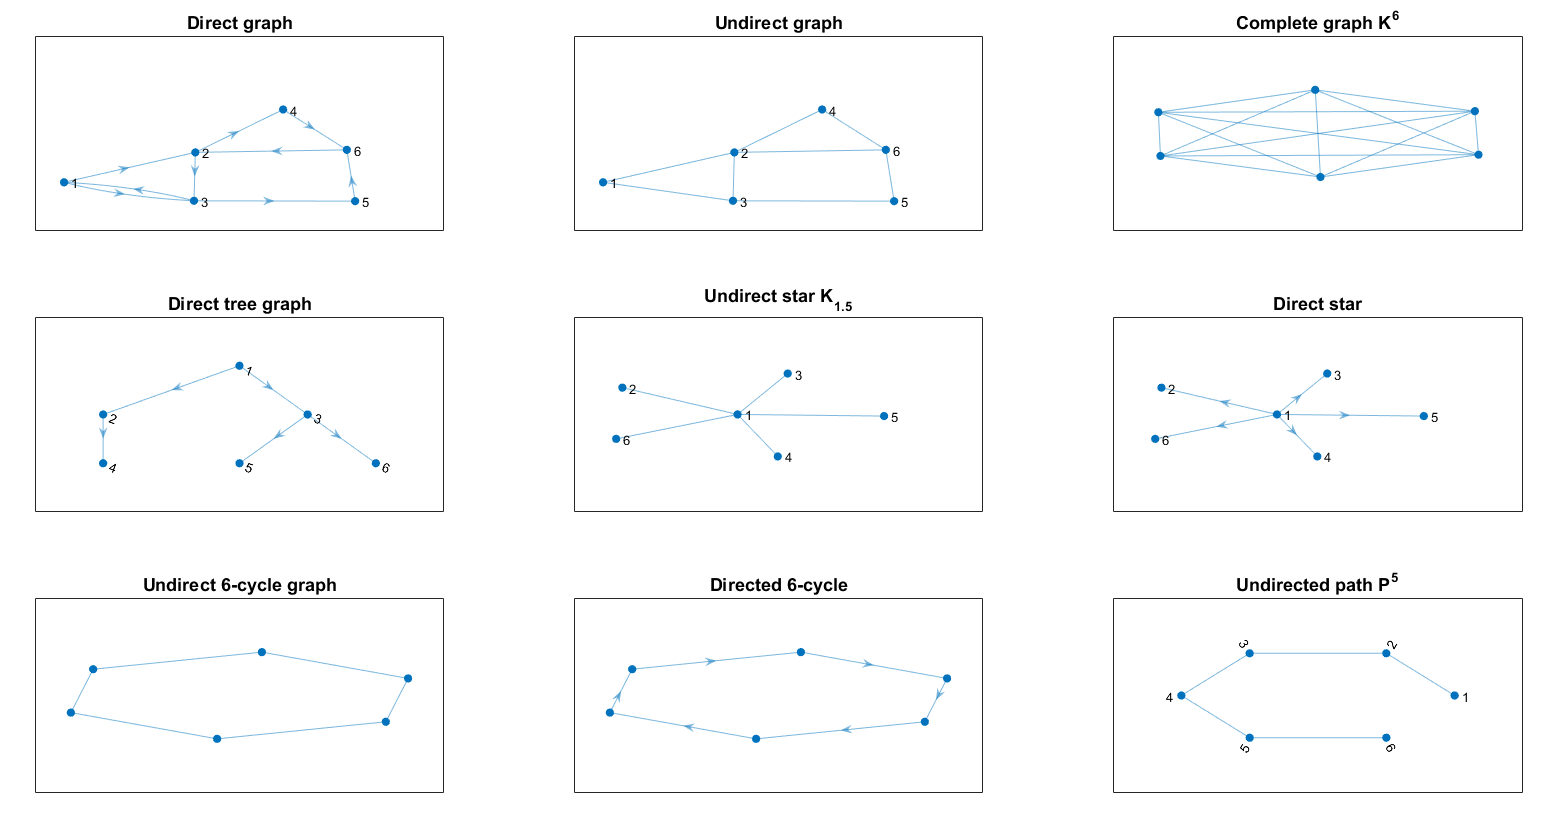
\includegraphics[scale=0.31]{figures/Graphs.png}
	\centering
	\caption{Graph topologies.}
	\label{graphs}
\end{figure}

Two different scalar single integrator dynamics of a local voting protocol, with agents were employed. First, we considered the following local voting protocol for every agent $i$
\begin{equation*}
u_i = \sum_{j \in N_i}a_{ij}(x_j-x_i)
\end{equation*}
with close-loop dynamics 
\begin{equation*}
\dot{x_i} = u_i,
\end{equation*}
which can be simplified as
\begin{equation*}
\dot{x_i} = -d_ix_i + [a_{i1}\hspace{.2cm}...\hspace{.2cm}a_{iN}]\begin{bmatrix}
x_1\\
.\\
.\\
.\\
x_N
\end{bmatrix}.
\end{equation*}
\vspace{.5cm}

The simulation plots are presented in figures \ref{cgt1}, \ref{cgt2} and \ref{cgt3}. The fastest graph that converges is the complete graph $K^6$, because each node is connected with all the others directly. Directed graph seem to converge slower than undirected, because the latter has nodes that considered to be connected in both directions. Moreover, for either directed star graph or directed tree graph all nodes converge to the leader, which remains to the initial state without changing during time. Furthermore, the undirected graph, the complete graph $K^6$, the undirected star $K_{1.5}$ graph, the undirected 6-cycle, the directed 6-cycle, and the undirected path $P^5$ converge to 0, while directed graph to non-zero value. Undirected graphs do not have oscillations to the path of converge, because they have real eigenvalues.

\begin{figure}[!h]
	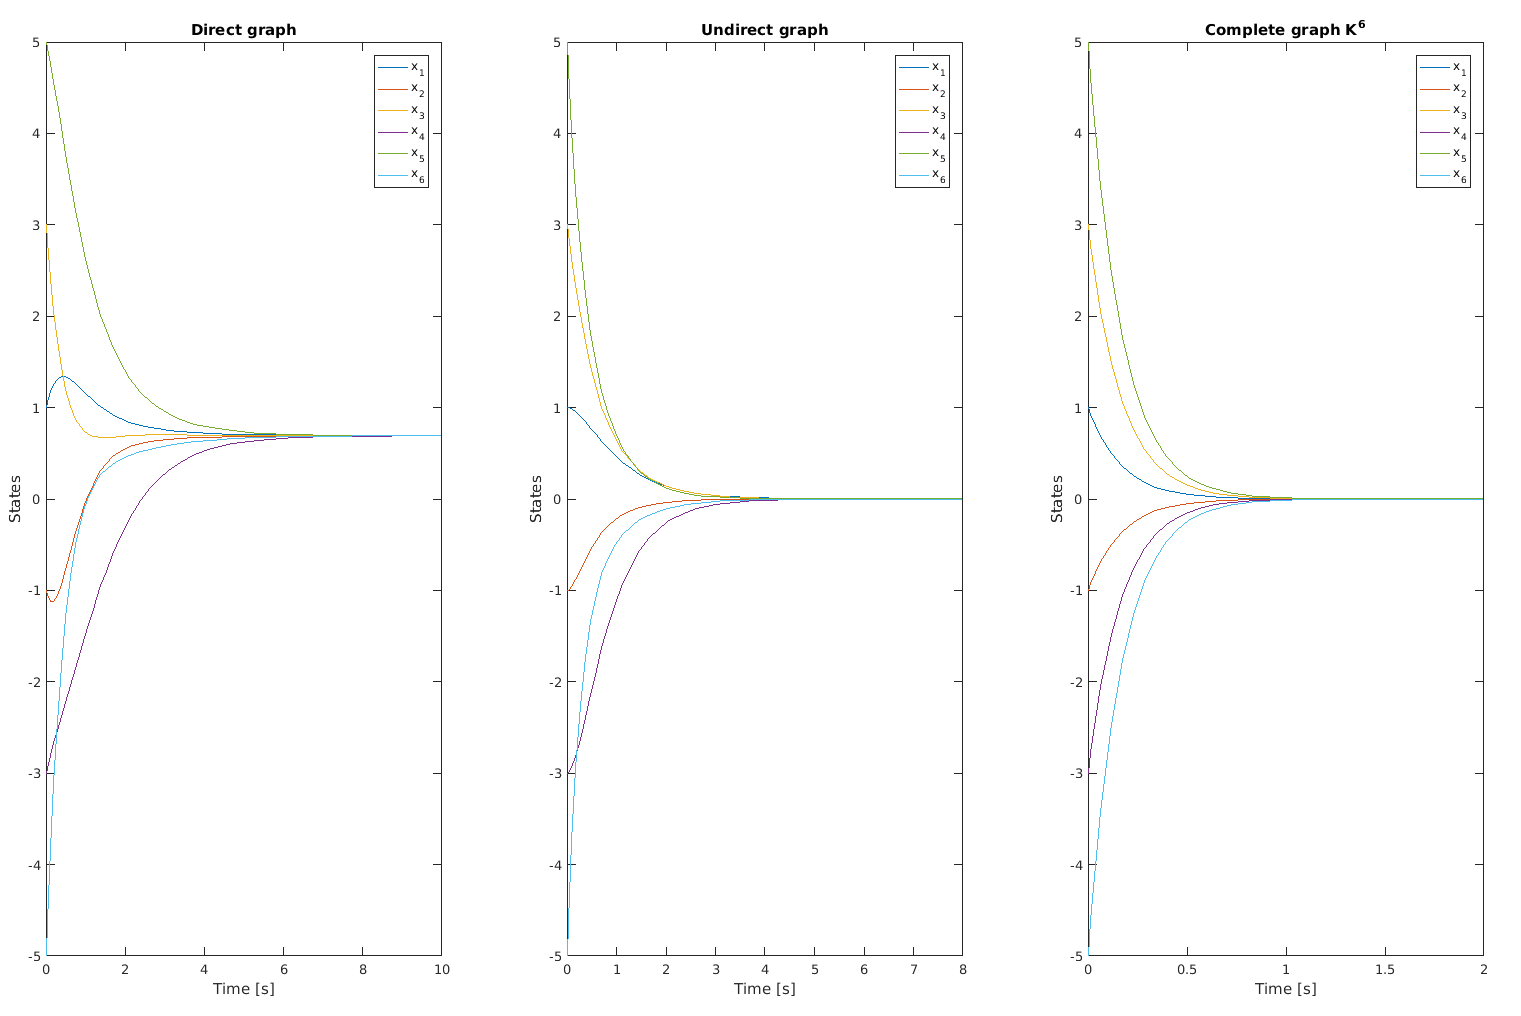
\includegraphics[scale=0.24]{figures/ConsensusGraphTopologies1.png}
	\centering
	\caption{Consensus plots for different graph topologies. Direct graph, undirect graph, and complete $K^6$ were studied.}
	\label{cgt1}
\end{figure}

Then, the motion of two graph topologies studied, with node dynamics for each agent $i$
\begin{equation*}
\dot{x_i}=Vcos(\theta_i),
\end{equation*}
\begin{equation*}
\dot{y_i}=Vsin(\theta_i),
\end{equation*}
\begin{equation*}
\theta_i = \sum_{j \in N_i}a_{ij}(\theta_j-theta_i).
\end{equation*}
In such case our state vector is $[x \hspace{.2cm} y \hspace{.2cm} \theta]^{\intercal}$. The plots of the simulations are presented in fig. \ref{cswarm}.

\begin{figure}[!h]
	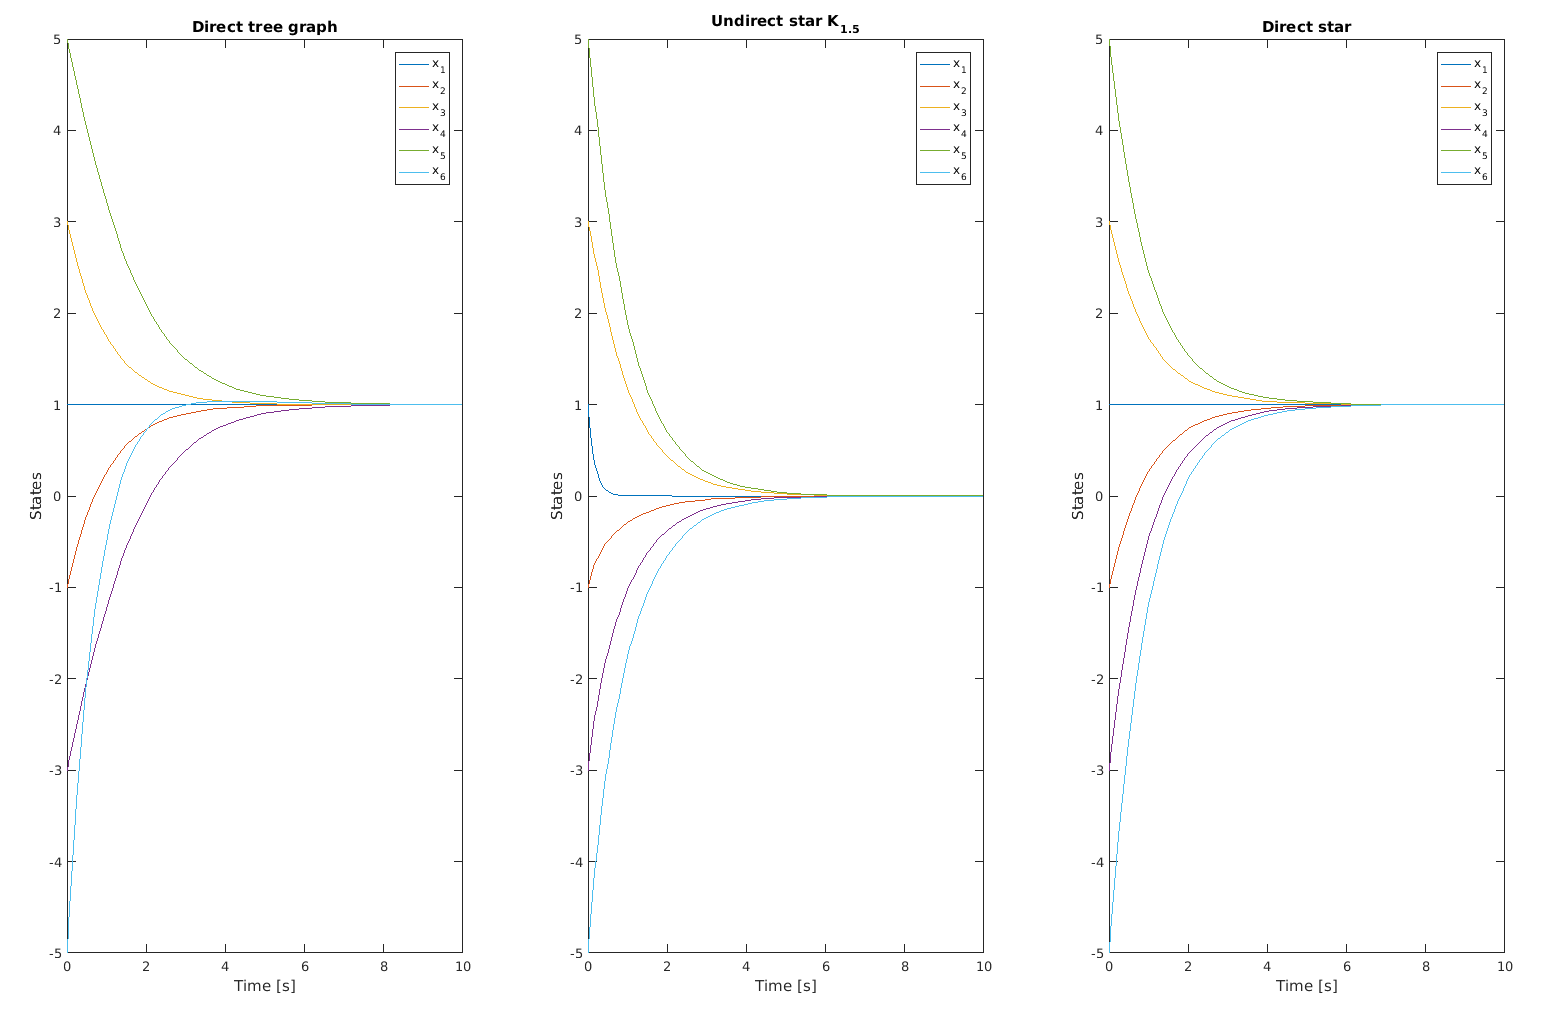
\includegraphics[scale=0.24]{figures/ConsensusGraphTopologies2.png}
	\centering
	\caption{Consensus plots for different graph topologies. Direct tree graph, undirect star $K_{1.5}$, direct star were studied.}
	\label{cgt2}
\end{figure}
\begin{figure}[!h]
	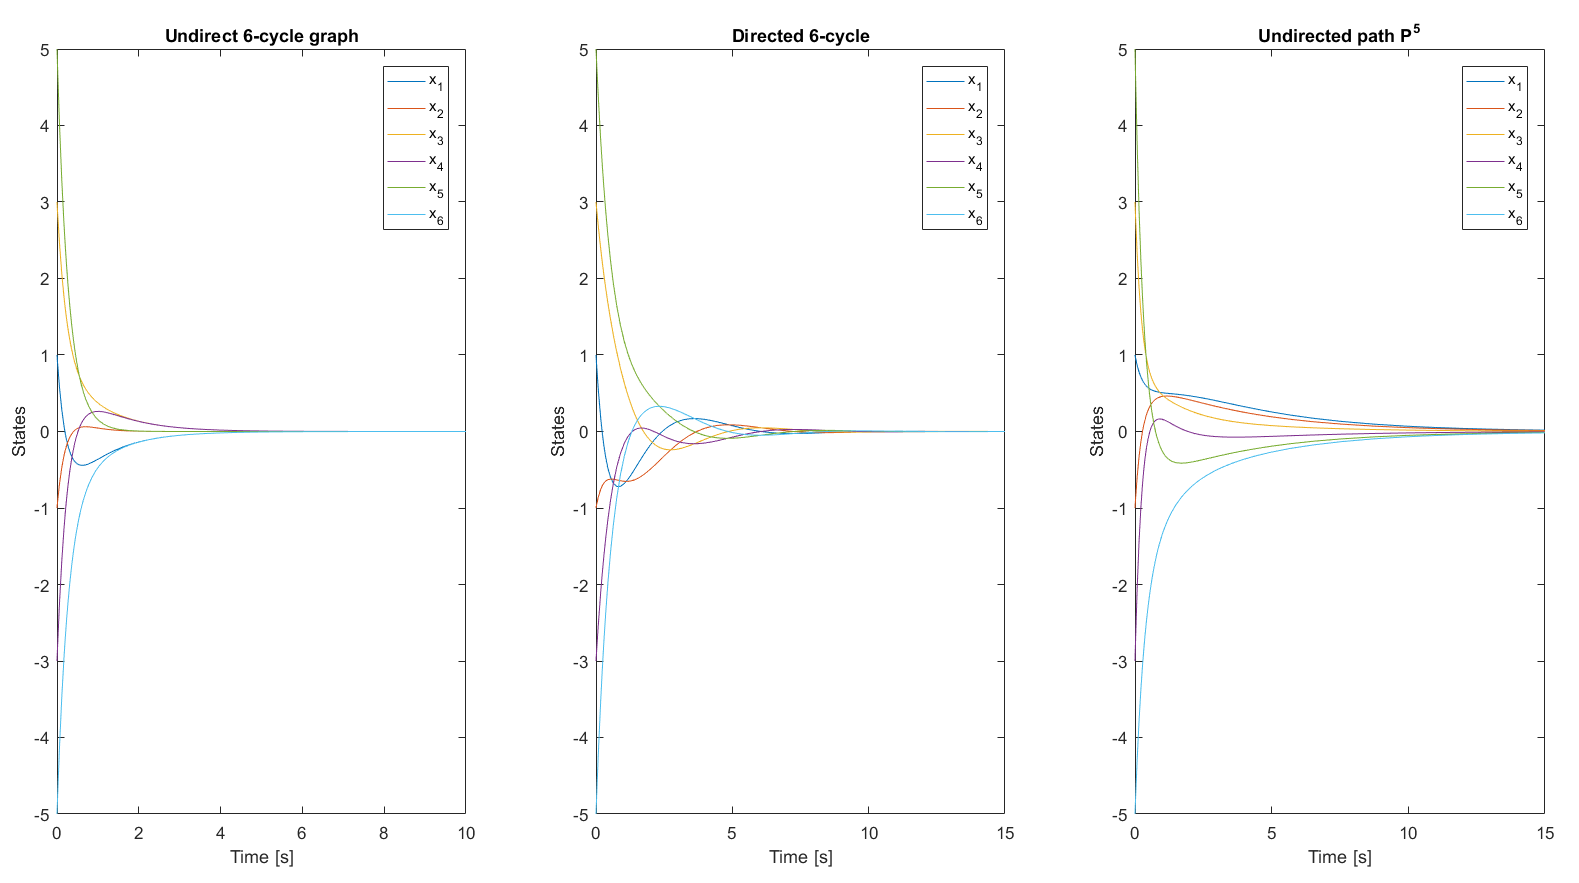
\includegraphics[scale=0.315]{figures/ConsensusGraphTopologies3.png}
	\centering
	\caption{Consensus plots for different graph topologies. Undirect 6-cycle graph, directed 6-cycle graph, and undirected path $P^5$ were studied.}
	\label{cgt3}
\end{figure}




The performance of the graph relies on the initial conditions. For the (x,y) plane all nodes started their path from the same point. The heading angle of the direct graph converges with many oscillations. All nodes of the direct graph at the Cartesian plane converge to the consensus heading node in the same direction and with the same orientation smoothly. The heading angle of the direct tree graph converges without oscillations and very fast given that the initial conditions were widely spread. All nodes of the direct tree graph at the Cartesian plane converge to the consensus heading node in the same direction and with the same orientation, but by surrounding the initial point at the beginning. 

\begin{figure}[!h]
	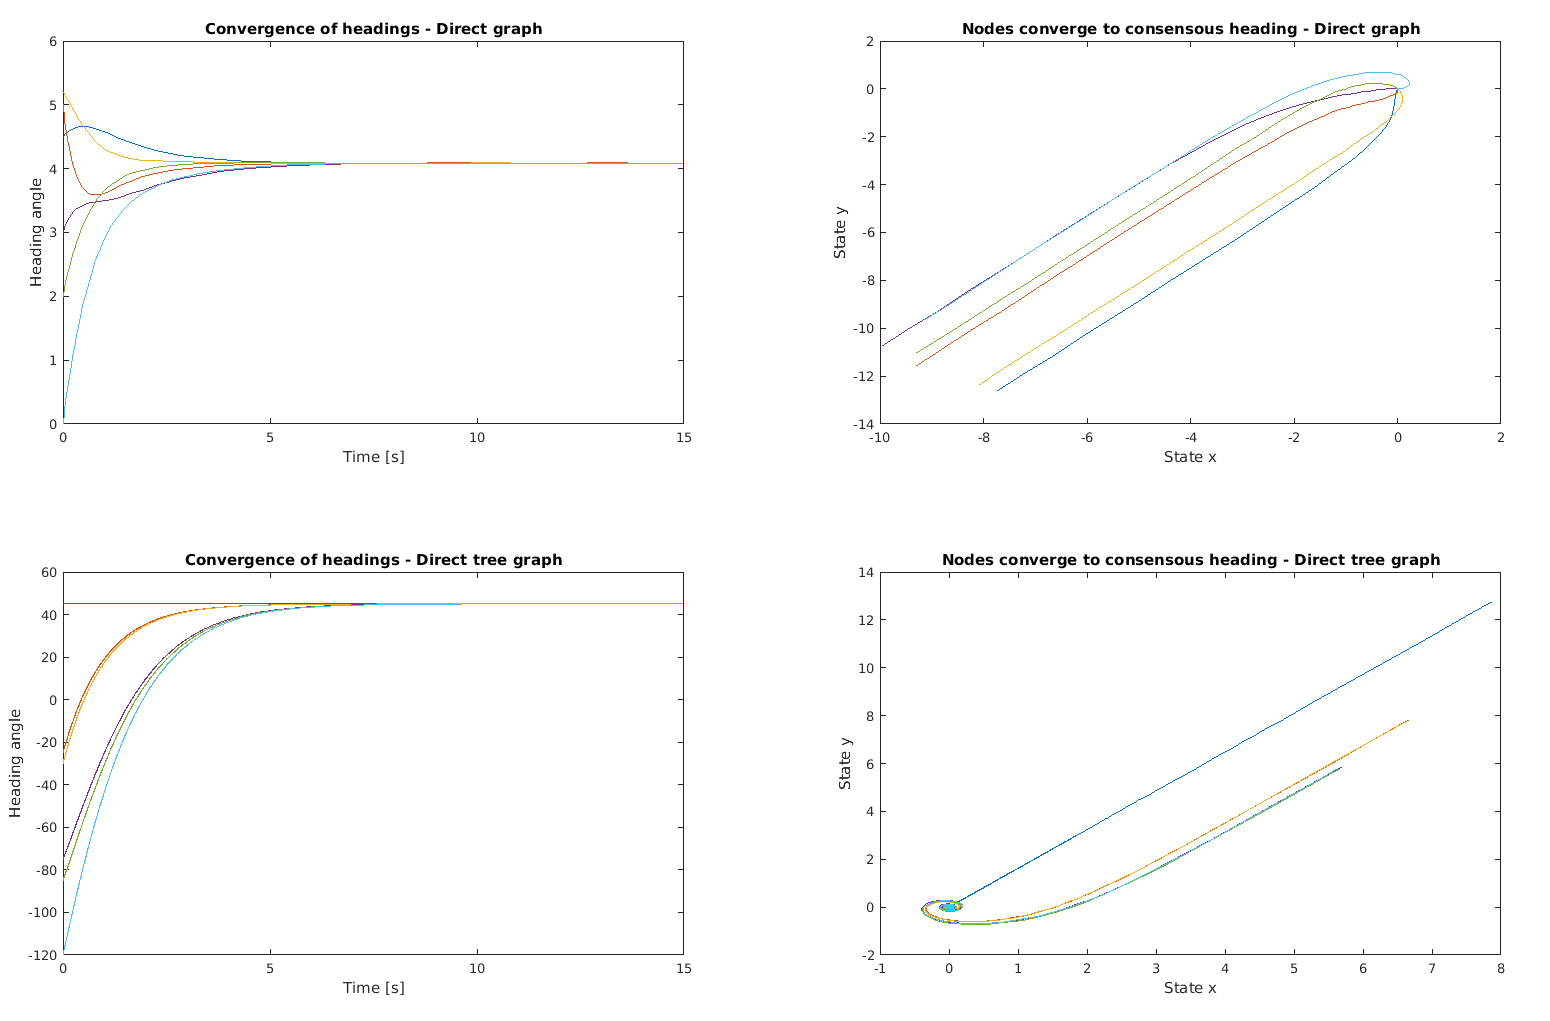
\includegraphics[scale=0.3]{figures/ConsensusSwarm.png}
	\centering
	\caption{Consensus of headings and motion consensus in (x-y) plane for direct and direct tree graph.}
	\label{cswarm}
\end{figure} 

\end{solution}

\end{document}


